% !TeX spellcheck = pl_PL-Polish
%%%%%%%%%%%%%%%%%%%%%%%%%%%%%%%%%%%%%%%%%%%%%%%%%%%%%%%%%
% Niniejszy plik przedstawia przykładowy skład 
% pracy dyplomowej na Wydziale Matematyki PWr. 
% 
% Autorzy: 
% Damian Fafuła
% Michał Kijaczko
% Jakub Michalczak
% Maciej Miśta
% Dagmara Nowak
% Tomasz Skalski
% Wojciech Słomian
%
%% Data utworzenia: 8.05.2018
% Numer wersji: 1
%
% Poniższą formatkę można rozpowszechniać i edytować 
% pod warunkiem zachowania numeru wersji, 
% informacji o autorach i dodaniu informacji 
% o wprowadzonych zmianach.
%
%%%%%%%%%%%%%%%%%%%%%%%%%%%%%%%%%%%%%%%%%%%%%%%%%%%%%%%%%
% Domyślną opcją jest: praca magisterska, język polski.
% W przypadku pracy pisanej w języku angielskim dodajemy 
% opcję [english].
% Dla pracy licencjackiej dodajemy opcję [licencjacka].
% Dla pracy inżynierskiej dodajemy opcję [inzynierska].
% Dopuszczalne są podwójne opcje, np. [licencjacka, english].
% Opcje dodajemy w kwadratowym nawiasie przy \documentclass.
%
%
%%%%%%%%%%%%%%%%%%%%%%%%%%%%%%%%%%%%%%%%%%%%%%%%%%%%%%%%%
\documentclass[inzynierska]{pwr_wmat_praca_dyplomowa}
%%%%%%%%%%%%%%%%%%%%%%%%%%%%%%%%%%%%%%%%%%%%%%%%%%%%%%%%%
%              DANE DO PRACY
%
% W przypadku pracy dyplomowej w języku angielskim nie jest konieczne 
% wypełnianie pól: \tytul{}, \kierunek{}, \specjalnosc{}, 
%                  \streszczenie{}, \slowakluczowe{}.
%%%%%%%%%%%%%%%%%%%%%%%%%%%%%%%%%%%%%%%%%%%%%%%%%%%%%%%%%
%
% Imię i nazwisko autora
\autor{Piotr Rogula}
%
% Tytuł pracy dyplomowej 
\tytul{Analiza statystyczna czasów na wykonywanie ruchów w
	szachach} 
\tytulang{Statistical analysis of times for making moves in chess}
%
% Tytuł / stopień / imię i nazwisko opiekuna
\opiekun{Prof. dr hab. inż. Marcin Magdziarz}
%
% Kierunek studiów wybieramy spośród następujących:
% 1) Matematyka
% 2) Matematyka i Statystyka
% 3) Matematyka stosowana
\kierunekstudiow{Matematyka Stosowana}
%
% Kierunek studiów po angielsku wybieramy spośród następujących:
% 1) Mathematics
% 2) Mathematics and Statistics
% 3) Applied Mathematics
\kierunekstudiowang{Applied Mathematics}
%
% Specjalność wybieramy spośród następujących: 
% KIERUNEK: Matematyka
% 1) Matematyka teoretyczna,
% 2) Statystyka matematyczna,
% 3) Matematyka finansowa i ubezpieczeniowa,
%
% KIERUNEK: Matematyka i Statystyka
% 4) Matematyka,
% 5) Statystyka i analiza danych, 
%
% 6) -- (w przypadku braku specjalizacji).
\specjalnosc{--} 
%
% Specjalność w języku angielskim wybieramy spośród następujących:
% KIERUNEK: Matematyka
% 1) Theoretical Mathematics,
% 2) Mathematical Statistics,
% 3) Financial and Actuarial Mathematics,
%
% KIERUNEK: Matematyka i Statystyka
% 4) Mathematics,
% 5) Statistics and Data Analysis,
%
% KIERUNEK: Applied Mathematics
% 6) Financial and Actuarial Mathematics, 
% 7) Mathematics for Industry and Commerce,
% 8) Computational Mathematics,
% 9) Modelling, Simulation and Optimization.
%
% 10) -- (w przypadku braku specjalizacji).
\specjalnoscang{--} 
%
% Krótkie streszczenia po polsku i angielsku
% - nie dłuższe niż 530 znaków.
\streszczenie{ROBOCZE: W pracy przeanalizowana zostanie zależność między czasami wykonania poszczególnych ruchów w szachach, a ich zgodnością z silnikiem szachowym. Zbadany zostanie rozkład tych czasów w zależności od poziomu graczy, na tej podstawie obliczone zostanie prawdopodobieństwo wykonania błędnego ruchu (max 530 znaków).}
\streszczenieang{Tutaj piszemy krótkie streszczenie pracy w języku angielskim (max 530 znaków).}
%
% Podajemy najważniejsze słowa kluczowe po polsku i angielsku
% - w obu przypadkach, nie więcej niż 150 znaków.
\slowakluczowe{ROBOCZE: analiza statystyczna, szachy, korelacja (max 150 znaków).}  
\slowakluczoweang{tutaj podajemy najważniejsze słowa kluczowe w języku angielskim (łącznie nie powinny być dłuższe niż 150 znaków)}
%
%
%%%%%%%%%%%%%%%%%%%%%%%%%%%%%%%%%%%%%%%%%%%%%%%%%%%%%%%%%
% Definicje, lematy, twierdzenia, przykłady i wnioski
% Komendy wywołujące twierdzenia, definicje, itd., 
% czyli 'theorem', 'definition', 'corollary', itd., 
% można zmienić wedle uznania.
\theoremstyle{plain}
\newtheorem{theorem}{Twierdzenie}
\numberwithin{theorem}{chapter}
\newtheorem{lemma}[theorem]{Lemat} 
\newtheorem{corollary}[theorem]{Wniosek}
\newtheorem{fact}[theorem]{Fakt}
\theoremstyle{definition}
\numberwithin{theorem}{chapter}
\newtheorem{definition}[theorem]{Definicja} 
\newtheorem{example}[theorem]{Przykład}
\newtheorem{note}[theorem]{Uwaga}
%%%%%%%%%%%%%%%%%%%%%%%%%%%%%%%%%%%%%%%%%%%%%%%%%%%%%%%%%


%%%%%%%%%%%%%%%%%%%%%%%%%%%%%%%%%%%%%%%%%%%%%%%%%%%%%%%%%
%%%%%%%%%%%%%%%%%%%%%%%%%%%%%%%%%%%%%%%%%%%%%%%%%%%%%%%%%
\begin{document}
\bibliographystyle{plain}
\frontmatter
\maketitle
\mainmatter
\tableofcontents
%\listoffigures
%\listoftables

{\backmatter \chapter{Wstęp}}
\textbf{We wstępie zapowiadamy, o czym będzie praca. Próbujemy zachęcić czytelnika do dalszej lektury, np. krótko informując, dlaczego wybraliśmy właśnie ten temat i co nas w nim zainteresowało.}

Wraz z rozwojem technologii komputerowej, rozpoczęła się nowa era szachów. Technologia korzystając z dużej mocy obliczeniowej, bezpowrotnie wyprzedziła człowieka w grach deterministycznych, do których zaliczają się szachy. Profesjonalni szachiści zaczęli wykorzystywać nowe strategie korzystając z coraz lepszych silników szachowych. Silniki te oceniają wprowadzoną pozycję pod kątem przewagi jednej ze stron. 

W dobie internetu gra w szachy stała się dużo wygodniejsza niż przed laty. Ludzie grają w różnych miejscach i praktycznie o każdej porze. W związku z tym dużo większą popularnością zaczęły cieszyć się szachy szybkie, czyli takie, w których każdy z zawodników ma relatywnie mało czasu na wykonanie wszystkich ruchów. Wiąże się to z dużo większym znaczeniem dysponowania czasem w trakcie gry. W każdym ruchu zawodnik musi ustalić równowagę pomiędzy dokładnością ruchu, a czasem, który jest w stanie na ten ruch poświęcić. 

Przedmiotem badań tej pracy jest analiza zależności między dokładnością ruchu, a czasem, który został na niego poświęcony dla zawodników prezentujących różny poziom umiejętności i dla różnych formatów czasowych.\textbf{ Zbadanie takiej zależności może pozwolić na określenie optymalnego czasu na wykonanie ruchu dla odpowiedniej fazy gry i formatu czasowego.}

\textbf{DODAĆ TUTAJ TROCHE I OGÓLNY CEL}\\


\textbf{W PIERWSZEJ CZĘŚCI - ZAGADNIENIA TEORETYCZNE DOTYCZĄCE SZACHÓW}\\
W pierwszej części pracy przedstawione i dość obszernie wyjaśnione zostaną podstawowe zagadnienia teoretyczne związane z szachami, systemami rankingowymi i silnikami szachowymi.


\textbf{W DRUGIEJ CZĘŚCI ZAGADNIENIA TEORETYCZNE ZE STATYSTYKI I METODOLOGII}\\
Kolejna część pracy opowiada o zagadnieniach teoretycznych z dziedziny statystyki, zastosowanych w analizie przedstawionych problemów.
 
 
\textbf{PÓŹNIEJ DOKŁADNE SFORMUOWANIE PROBLEMU}\\
Główna część pracy zawiera przedstawienie zależności...

\textbf{DOKŁADNE ROZWIĄZANIE PROBLEMU}\\
a póżniej rozwiązanie...

\textbf{PODSUMOWANIE}\\
W końcowej części pracy [...] podsumowanie, wnioski...

\chapter{ZAGADNIENIE TEORETYCZNE I - DOTYCZĄCE SZACHÓW}
Niniejszy rozdział poświęcony zostanie zagadnieniom teoretycznym dotyczącym szachów, używanych systemów rankingowych oraz działaniu silników szachowych.
\section{ZASADY GRY W SZACHY}
Początki szachów nie są znane, jednak ich historia trwa już ok. 1500 lat i zaczyna się w Indiach. Na przestrzeni wieków zasady gry w szachy były wielokrotnie zmieniane. Powszechnie stosowane przepisy pochodzą z roku 1851.\\

\textbf{krótko na czym polegają szachy i cite gdzie można znaleźć pełne przepisy,isbn:002028540X}\\

Gra odbywa się na kwadratowej planszy o wymiarach 8 na 8 pól. Każdy gracz posiada 16 figur, ustawionych w pozycji startowej i stojących po przeciwnych stronach szachownicy. Zawodnicy wykonują na przemian ruchy dowolną ze swoich figur, zgodnie z jej zasadami poruszania się. W trakcie tury zawodnikowi upływa czas ustalony przed grą. W niektórych wariantach gracz otrzymuje też niewielką ilość czasu za wykonanie każdego ruchu.\\

Wygrana następuje, gdy król jednego z graczy jest atakowany i nie można w legalny sposób nim ruszyć, ani zasłonić jedną ze swoich figur przed atakiem. Pozycję taką nazywa się ,,matem'' Drugim sposobem na wygranie jest skończenie się czasu jednego z graczy, niezależnie od sytuacji na szachownicy. 
Gra może też zakończyć się remisem. Następuje on, gdy żaden z graczy nie ma na planszy figur, które mogą pozwolić na ,,zamatowanie'' przeciwnika. Inną możliwością jest trzykrotne powtórzenie się na planszy tej samej pozycji. Do remisu doprowadza też sytuacja, w której jednemu z graczy zakończył się czas, a jego przeciwnik nie ma figur pozwalających na wygraną lub gdy jeden z graczy nie ma możliwości wykonania żadnego legalnego ruchu, a jego król nie jest atakowany.

W związku z możliwością przegranej poprzez upłynięcie czasu na zegarze, zawodnicy muszą indywidualnie określić podczas gry, ile czasu są w stanie poświęcić danemu ruchowi, tak by nie stracić na niego zbyt wiele czasu, ale też, żeby ruch był jak najlepszy, co jest przedmiotem badań niniejszej pracy.

\section{OPISAĆ NOTACJĘ szachową????? - nie będę w sumie nic z nią robić, ale jest}

\section{System rankingowy Glicko-2}
\textbf{opisać ogólnie troche historii o systemach rankingowych?}
System rankingowy ELO - pierwowzór systemu Glicko-2, został zaprezentowany w latach pięćdziesiątych dwudziestego wieku przez Węgierskiego fizyka i szachistę Arpada Elo (1903-1992) \textbf{[CITE]}. Początkowo był używany jedynie w szachach, jednak wraz ze wzrostem jego popularności zaczął być stosowany również w innych rozgrywkach z możliwością pomiaru poziomu zawodników. System ten jest pierwszym systemem mającym podłoże probabilistyczne i jest oparty na rozkładzie normalnym z ustaloną średnią. Przyznaje odpowiednią liczbę punktów zwycięzcy rozgrywki i odbiera przegranemu bazując na różnicy między ich aktualnym rankingiem.


System Glicko-2 używany przez stronę \textbf{Lichess.com}, na danych której oparta jest niniejsza praca, opracowany został przez Marka Glickmana jako ulepszenie systemu ELO. Podstawową zmianą jest uwzględnienie historycznych wyników każdego z zawodników w celu ustalenia wariancji aktualnego rankingu. Glickman w swojej pracy z roku 1998 \textbf{[cite]} przedstawia problem dwóch graczy o takim samym rankingu, z których jeden gra regularnie, a drugi wrócił do gry po długiej przerwie. System Glicko-2 przyznając punkt za grę bierze pod uwagę wiarygodność każdego z rankingów. Zawodnikowi grającemu regularnie zostanie przyznane bądź odebrane mniej punktów ze względu na duże potencjalne odchylenie rankingu przeciwnika od zadeklarowanej wartości. Innymi słowy, w miarę zwiększania się liczby partii gracza, przedział ufności dla jego realnego rankingu zawęża się i przypisany mu ranking zbiega do realnego poziomu i wiarygodność przypisanego rankingu jest uwzględniaan w przyznawaniu i odbieraniu punktów zawodnikom po zakończeniu partii.

\textbf{WRZUCIĆ MATEMATYKĘ STOJĄCĄ ZA GLICKO-2???}
x

\textbf{Tutaj jakiś wykresik może jak wygląda rozkład rankingu zawodników na platformie Lichess ???}
\section{Funkcja oceny}
Przed przystąpieniem do opisania funkcji, należy wytłumaczyć działanie silnika szachowego, który dokonuje oceny pozycji.
\subsection{Stockfish}
Stockfish jest jednym z najlepszych i najpopularniejszym obecnie używanym silnikiem szachowym, którego zaprojektowali Joost VandeVondele, Joon Kiiski, Marco Costalb, Tord Romstad, Gary Linscott, Stefan Geschwentner i Stéphane Nicolet i stale ulepszany jako oprogramowanie typu open-source. Strona \textbf{Lichess.com}\cite{stockfish_lichess} tak jak większość stron internetowych poświęconych szachom on-line, wykorzystuje go do analizy i oceny aktualnej pozycji.

Stockfish poprzez przeszukiwanie wg strategii mini-max z odcięciem, za pomocą algorytmu alfa-beta, analizuje legalne (czyli następujące po ruchu zgodnym z zasadami gry) pozycje, które mogą wyniknąć z aktualnej sytuacji na szachownicy. Dobierają na podstawie najlepszego możliwego zestawu ruchów (zakłada się, że każdy z graczy wykona najlepszy w ocenie silnika ruch) pozycje, które wystąpią dla określonej głębokości (głębokość 18 oznacza 18 ruchów białych i 18 czarnych wykonanych zaczynając z analizowanej pozycji) i na ich podstawie ocenia aktualną pozycję, określając przewagę jednego z graczy

\subsection{Ewaluacja}
Wspomniana wcześniej ewaluacja, wyliczana przez silnik szachowy jest wynikiem liniowej funkcji 
ważonej sumy cech, na którą składają się między innymi:\\
$f_b,f_c$ oznaczających wartość figur odpowiednio białych i czarnych\\
$k_b,k_c$ oznaczających bezpieczeństwo króla odpowiednio białych i czarnych\\
$m_b,m_c$ oznaczających mobilność figur odpowiednio białych i czarnych\\
$z_b,z_c$ oznaczających potencjalne zagrożenia wykonane odpowiednio białych i czarnych\\


Funkcję można dla zapewnienia intuicji zapisać w uproszeniu:
\begin{equation}
	f(f_b,f_c,k_b,k_c,m_b,m_c,\dots)=c_1(f_b-f_c)+c_2(k_b-k_c)+c_3(m_b-m_c)+\dots
\end{equation}
gdzie:
$c_i$ są stałymi określającymi wagę danej pary zmiennych.

Wraz ze wzrostem wartości funkcji zwiększa się przewaga białych, natomiast wraz z jej spadkiem, przewaga czarnych. Wartość wynosząca 0 oznacza stan równowagi, czyli sytuacji, w której żadna ze stron nie ma przewagi lub gracz z gorszą sytuacją na szachownicy jest w stanie przy odpowiedniej kombinacji ruchów doprowadzić do remisu. Dodatkowo, w przypadku nieuniknionego zwycięstwa jednej ze stron w \textit{n} ruchach, wynikiem funkcji zamiast odpowiedniej wartości liczbowej jest tekst \textit{\#-n} w przypadku wygranej czarnych lub \textit{\#n} w przypadku wygranej białych, oznaczający nieuchronną wygraną jednego z graczy po wykonaniu \textit{n} ruchów, przy najlepszej obronie przeciwnika.


\subsection{rodzaje błędów szachowych} \label{sec:mysection}

% https://en.wikipedia.org/wiki/Chess_annotation_symbols

W notacji szachowej obok zapisanego ruchu mogą pojawić się symbole określające jakość danego ruchu. Dla analizowanych danych, ruch oceniany jest przez silnik szachowy za pomocą skomplikowanych algorytmów, których głównym składnikiem jest zmiana oceny pozycji na szachownicy przez silnik.
Przykładowo, gdy przed ruchem czarnych ocena pozycji wynosiła -2, a po ruchu 3, silnik oceni ruch jako duży błąd, jednakże jeśli wcześniejsza ocena wynosiła -18, a po ruchu -13, silnik nie oznaczy ruchu jako błędny, ponieważ przewaga czarnych i tak jest bardzo duża.

Wśród licznych oznaczeń silnika, w pracy analizowane będą następujące oznaczenia\textbf{[cite: Corpus ID: 53767853 Secrets of Rook Endings J. Nunn Published 1992 Computer Science]}:
\begin{itemize}
	\item ??\hphantom{!} -- duży błąd (ang. \textit{blunder})
	\item ?\hphantom{?!}  -- pomyłka (ang. \textit{mistake})
	\item ?!\hphantom{?} -- niedokładność  (ang. \textit{innacuracy})
\end{itemize}




\chapter{ZAGADNIENIE TEORETYCZNE II - użyte metody, teoria stojąca za rozwiązaniami problemów}
Niniejszy rozdział poświęcony zostanie zagadnieniom teoretycznym z dziedziny statystyki, zastosowanych w analizie przedstawionych problemów.
\section{zagadnienie 1...}

\chapter{sformułowanie i rozwiązanie problemów analitycznych}
\section{sformułowanie problemów}
Podstawowym problemem podjętym w pracy jest analiza zależności pomiędzy czasem na wykonanie ruchu, a jego dokładnością. Główny nacisk kładziony zostanie na ruchy oznaczone przez silnik jako ,,duży błąd'', co można uargumentować tym, że właśnie te ruchy mają największy wpływ na grę, szczególnie biorąc pod uwagę szachy szybkie, gdzie czasu na ruch jest zdecydowanie mniej, czego wynikiem jest to, że takie ruchy pojawiają się znacznie częściej. Dodatkową osią ujętą w rozważaniach będzie ranking zawodników i jego wpływ na rozkłady danych. Sprawdzona i wzięta pod uwagę zostanie również zależność między numerem ruchu, a czasem na wykonanie oraz jego dokładnością.
Zwieńczeniem pracy będzie podjęcie próby wyznaczenia optymalnego czasu na wykonanie ruchu, tak, by zminimalizować ryzyko popełnienia dużego błędu.

\section{Dane}
Dane potrzebne do analizy zostały pobrane z platformy Lichess \cite{lichess}. Są one przechowywane w pliku o rozmiarze ponad 72 Gb. Zawiera on wszystkie gry (ponad 35 milionów) rozegrane na platformie w maju 2019 roku. Ponadto, ok. 7\% gier zostało wcześniej przeanalizowane przez silnik szachowy Stockfish i posiadają dane punktowe o nazwie \textit{Eval}, określające unormowaną przewagę jednego z graczy oraz określenie części ruchów przez silnik jako błędne. Dodatkowo silnik określa jakość wykonanego ruchu wg własnych kryteriów (opisane w sekcji \ref{sec:mysection} na stronie \pageref{sec:mysection}). Przykładowy zapis jednej takiej gry z pliku został zaprezentowany na rysunku \ref{rys:zapis_gry}. Informacje potrzebne do analizy to:
\begin{itemize}
	\item WhiteElo -- ranking białych
	\item BlackElo -- ranking czarnych
	\item TimeControl -- czas na wykonanie ruchów każdego z graczy w formacie  ,,sekundy + sekundy dodane za wykonanie ruchu''
	\item \% eval -- aktualna przewaga jednej ze stron
	\item zapis partii ze wskazaniem błędnych ruchów w ocenie silnika
	\item \% clk -- pozostały czas w formacie ,,godziny : minuty : sekundy''
	\item result -- wynik partii
\end{itemize}

\begin{figure}[H]
	\centering
	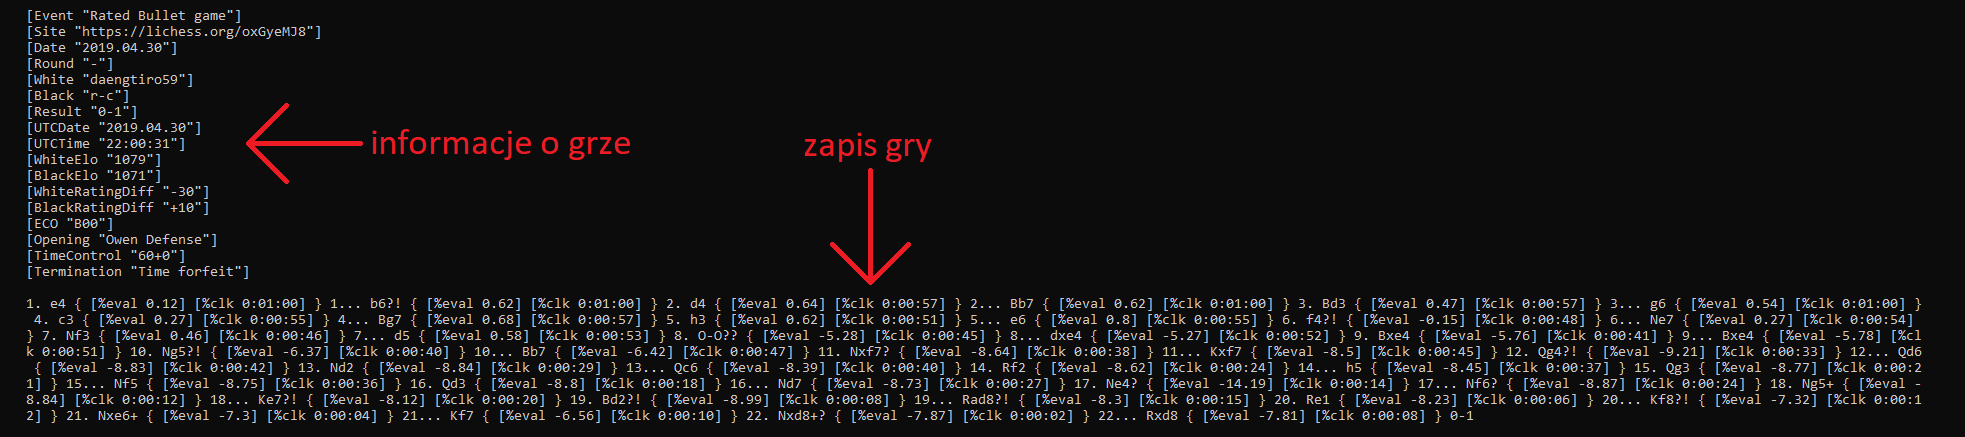
\includegraphics[width=\textwidth]{zapis_gry.png}
	\caption{Przykładowy zapis jednej partii zawierającej ocenę silnika Stockfish}
	\label{rys:zapis_gry} 
\end{figure}

Istotnym problemem związanym z danymi jest dokładność pozostałego czasu jedynie do sekund, co zaburza lekko ich istotę, szczególnie podczas analizy gier w krótszym formacie czasowym, gdzie części sekundy są bardziej znaczące. Dodatkowo ruch, który oznaczony został jako n sekund w rzeczywistości jest ruchem z przedziału obustronnie otwartego (n-1,n+1) sekund. Przy większej liczbie danych nie ma to jednak większego znaczenia, ponieważ zgodnie z Prawem Wielkich Liczb można takie dane uśrednić do \textit{n}. Jedynym problemem, który może się pojawić jest późniejsze sprawdzenie zgodności danych z rozkładem. 

\subsection{Odfiltrowanie danych}

Pierwszym krokiem potrzebnym do wykonania analizy jest odfiltrowanie danych.
Po rozdzieleniu pliku tekstowego na kolejne gry, pozostawione zostały jedynie te, które zostały wcześniej ocenione przez silnik. Następnie dla każdej z nich przeanalizowany został każdy ruch, do którego zostały przypisane następujące atrybuty:
\begin{itemize}
	\item score -- ocena ruchu wg silnika Stockfish
	\item WhiteElo -- ranking białych
	\item BlackElo -- ranking czarnych
	\item TimeControl -- czas na wykonanie ruchów każdego z graczy w formacie  ,,sekundy + sekundy dodane za wykonanie ruchu''
	\item color -- gracz, wykonujący dany ruch
	\item move -- numer ruchu w danej partii
	\item result - wynik partii
\end{itemize}

Stworzona baza zawiera 9 737 663 posunięć ze 154 981 gier, co daje średnią 31.41 ruchu na grę (jeden ruch oznacza posunięcie białych i czarnych). Fragment bazy przedstawiony został na rysunku \ref{rys:baza_ruchow}. 
\begin{figure}[H]
	\centering
	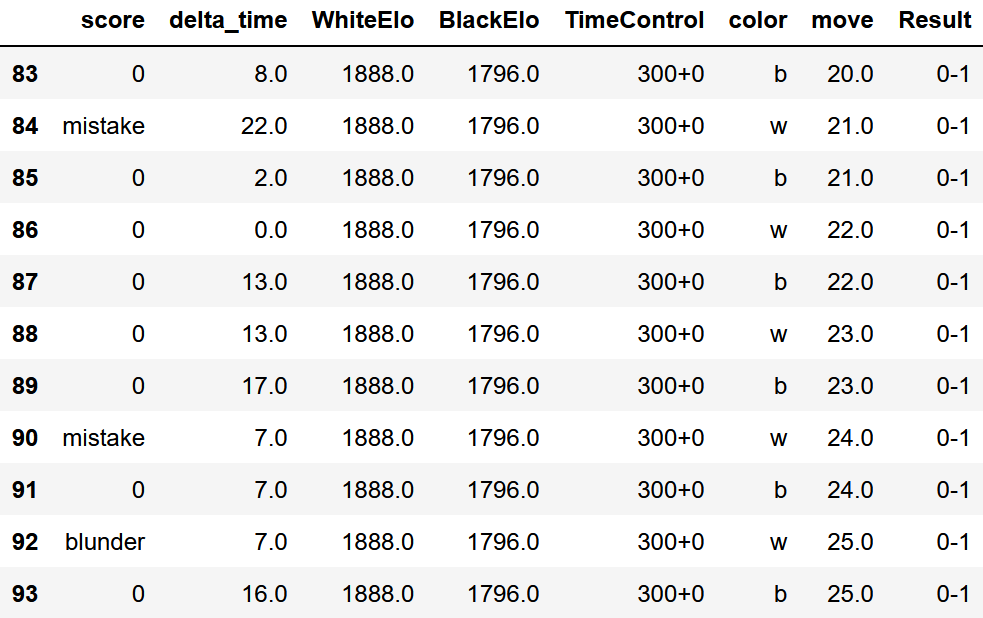
\includegraphics[width=\textwidth]{danee.png}
	\caption{fragment bazy ruchów wraz z oceną silnika}
	\label{rys:baza_ruchow}
\end{figure}



\section{Analiza pierwszego problemu}
Pierwszym problemem, który zostanie poruszony jest zbadanie statystycznej zależności jakości wykonanego ruchu wg oceny silnika Stockfish od czasu potrzebnego na jego wykonanie. W celu uzyskania bardziej precyzyjnych wyników pierwsze 4 ruchy (zarówno białych jak i czarnych) nie będą brane pod uwagę. Są one elementem teorii otwarć szachowych [\textbf{ref ISBN 0-19-280049-3}], w związku z czym wykonywane są zazwyczaj bardzo szybko i ze znikomą szansą popełnienia błędu, co może spowodować zaburzenie danych. Dodatkowo na stronie Lichess.com pierwszy ruch obydwu zawodników zawsze zabiera 0 sekund.

\begin{table}[H]
	\caption{baza ruchów z gier na portalu Lichess z maja 2019, 6 najpopularniejszych formatów}
	\centering
	\begin{tabular}{|l|r|}
		\hline
		\multirow{2}{*}{\begin{tabular}[c]{@{}l@{}}Format czasowy \\ sekundy+sekundy przyznawane po wykonaniu ruchu\end{tabular}} & \multirow{2}{*}{\begin{tabular}[c]{@{}l@{}}liczba ruchów \\ w bazie\end{tabular}} \\
		&                                                                                   \\ \hline
		600+0 & 1 813 841\\
		300+0 & 1 409 904\\
		\hphantom{0}60+0 & 1 251 388 \\
		900+15 & 1 104 458 \\
		180+0 & 1 057 292\\
		300+3 & 941 262\\  \hline
	\end{tabular}
	\label{tab:formaty} 
\end{table}

W pracy, analizowane będzie sześć najpopularniejszych formatów czasowych granych na platformie Lichess. Są one przedstawione w tabeli \ref{tab:formaty}. Przy analizie z uwzględnieniem rankingu graczy, zastosowane będą podziały kwartylowe wg rankingu białych, rozkład rankingu wraz z zaznaczonymi kwartylami pokazany jest na rysunku \ref{rys:rozklad_elo}. Jak widać zbiega on do rozkładu normalnego. Anomalia dla rankingu 1500 związana jest z tym, że jest to ranking przyznawany każdemu graczowi przy jego pierwszej rozgrywce na platformie.
\begin{figure}[H]
	\centering
	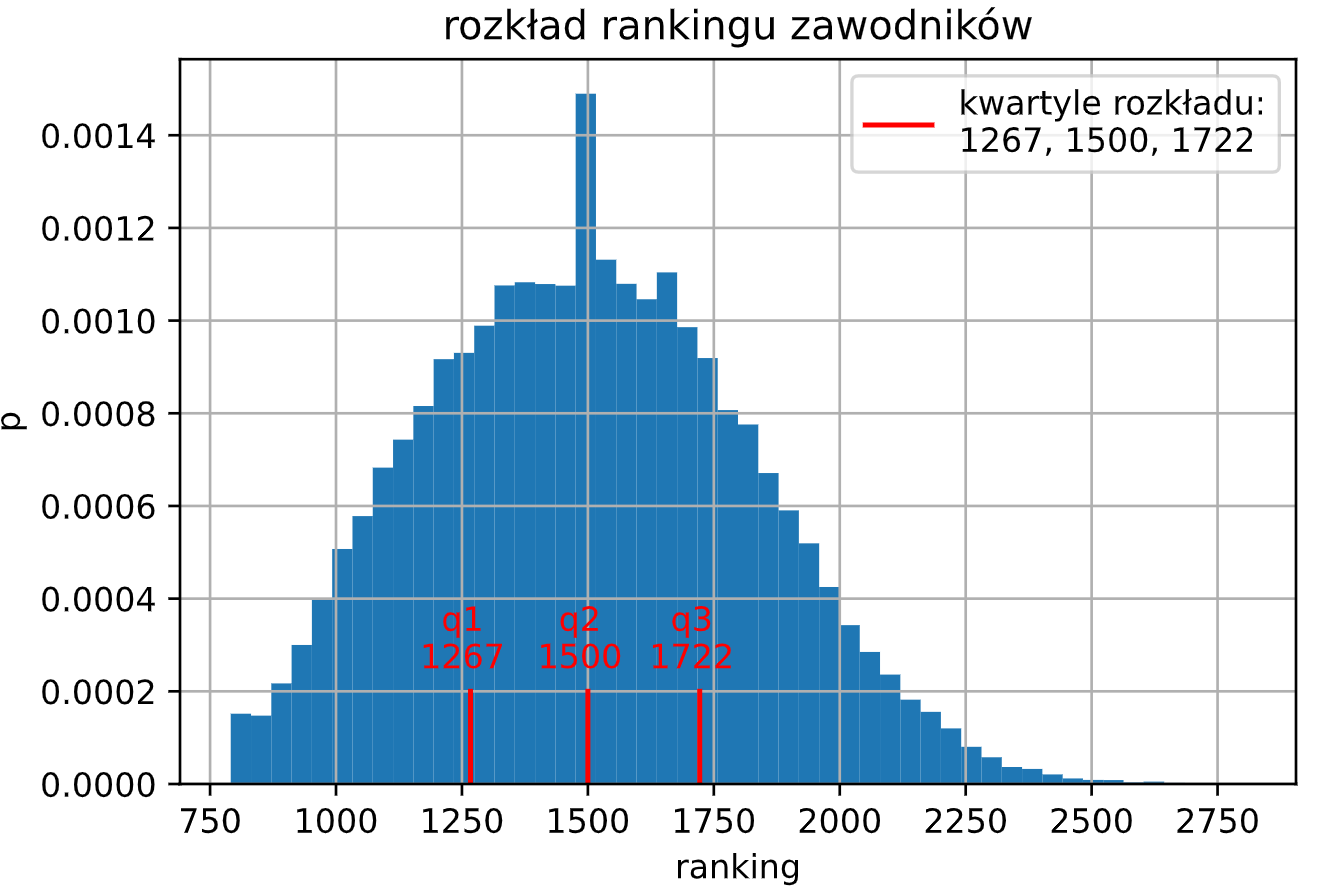
\includegraphics[width=\textwidth]{ranking.png}
	\caption{rozkład rankingu zawodników wraz z zaznaczonymi kwartylami}
	\label{rys:rozklad_elo}
\end{figure}


Po przyjrzeniu się danym można zauważyć, że pochodzą one z rozkładu logarytmicznie-normalnego, co można uwarunkować tym, że w zdecydowanej większości pozycji zawodnik potrzebuje chwili na odpowiedź na ruch przeciwnika, tj 



TUTAJ rozkłady, 	

np dla formatu 60+0 (60 sekund, brak dodawanego czasu po wykonaniu ruchu)

\begin{figure}[H]
	\centering
	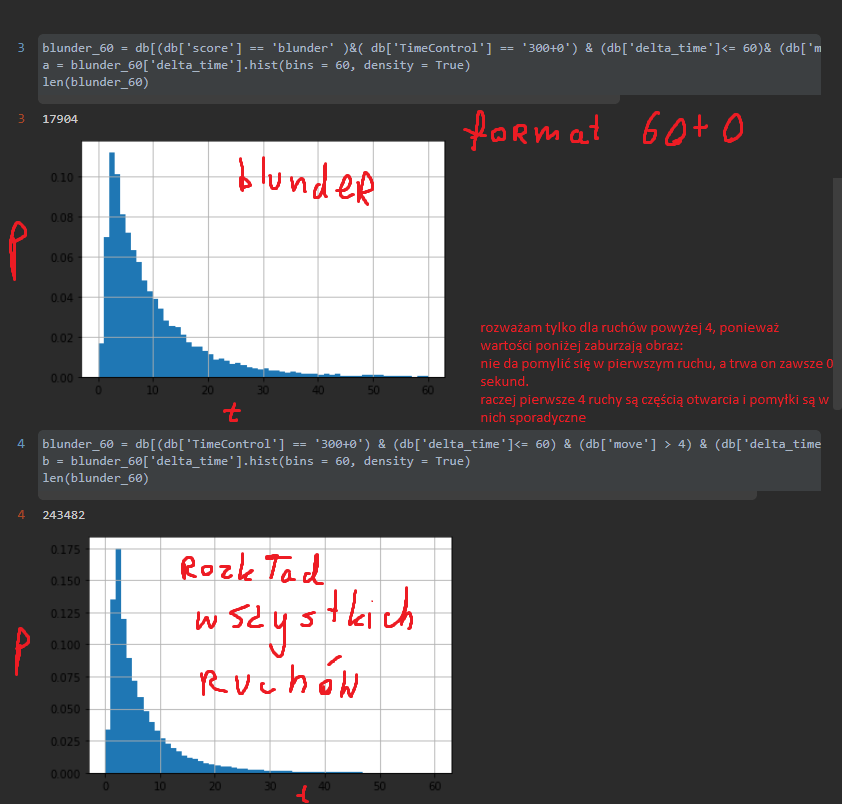
\includegraphics[width=\textwidth]{sample60.png}
	\caption{xxx}\label{xxx}
\end{figure}


oś x -> czas

oś y -> nieznormalizowana liczba ruchów typu 'blunder' (te najcięższe pomyłki)\newline


rozkład gamma... (?)\newline 




TO DO: 

sprawdzenie zmian dla rankingu graczy, różnicy rankingu graczy

porównanie z czasem na wykonanie każdego ruchu\newline



TO DO: 

czy różnica pomiędzy formatem z dodawanym czasem po ruchu, a bez dodawanego czasu jest widoczna?



\section{analiza drugiego problemu...}
tutaj statystyczne prawdopodobieństwo wykonania złego ruchu pod warunkiem poświęceniu mu konkretnego czasu,\newline

np, w formacie czasowym 60+0 na ruch zostały poświęcone 4 sekundy, jaka jest szansa, że został popełniony błąd \newline
\begin{figure}[H]
	\centering
	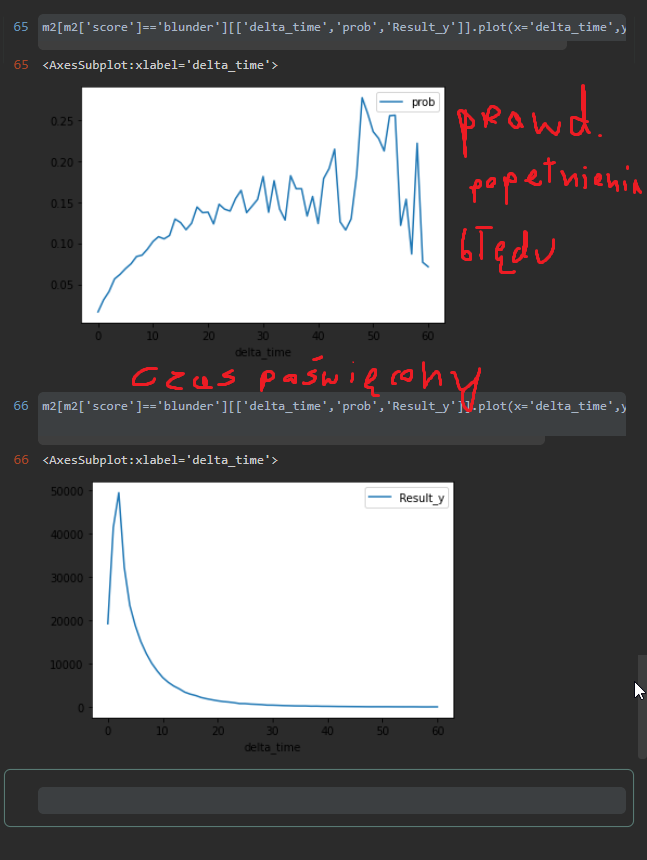
\includegraphics[width=\textwidth]{p_od_czasu.png}
	\caption{aaa}\label{aaa}
\end{figure}
CEL: 
ile powinno się poświęcić czasu na ruch by obniżyć prawdopodobieństwo wykonania błędu?\newline

\textbf{Tego jeszcze nie analizowałem}




\section{analiza trzeciego problemu...  and so on...}
w którym ruchu jest największa szansa na popełnienie błędu?
dla wszystkich rang
\begin{figure}[H]
	\centering
	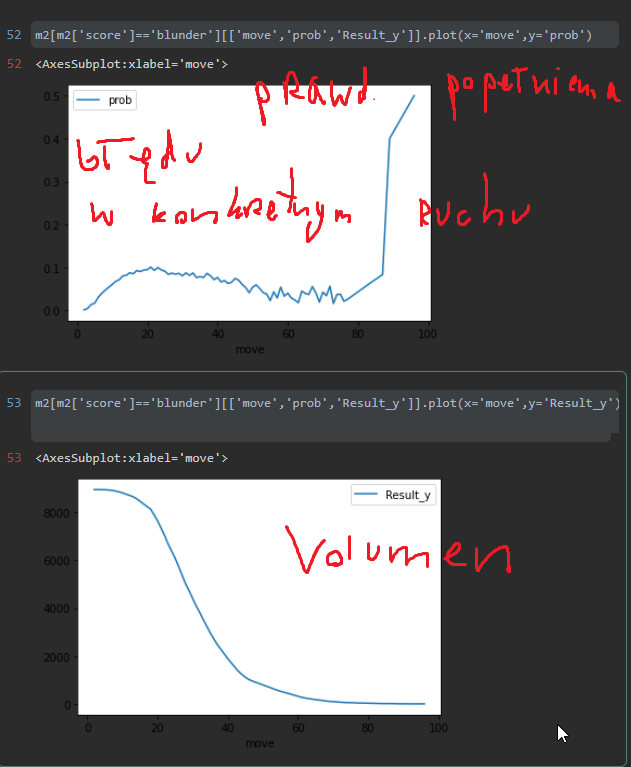
\includegraphics[width=\textwidth]{p_od_ruchu.png}
	\caption{aaa}\label{aaa}
\end{figure}
\chapter{wnioski, podsumowanie}

\chapter{tabelka}
Tabela \ref{tab:przykladowa} 
\begin{table}[H]
	\caption{Podstawowa Tabela}
	\centering
	\begin{tabular}{ccc}
		\hline
		\hline                       
		Państwo & PKB (w milionach USD )& Stopa bezrobocia  \\  [0.5ex] 
		\hline 
		Stany Zjednoczone & 75 278 049 & 4,60\%  \\
		Chiny & 11 218 281 & 4,10\%   \\
		Japonia & 4 938 644 & 3,10\%  \\
		Niemcy & 3 466 639 & 6,00\%   \\
		Wielka Brytania & 2 629 188 & 4,60\%  \\ [1ex]  
		\hline 
	\end{tabular}
	\caption*{\textit{Źródło: opracowanie własne}}
	\label{tab:przykladowa2} 
\end{table}
\chapter{rysunek}
Rysunki do pracy dyplomowej należy wstawiać w sposób podobny do wstawiania tabel, z~zasadniczą różnicą polegającą na tym, że podpis powinno umieszczać się centralnie pod rysunkiem, a nie powyżej niego. Numeracja i sposób cytowania pozostają bez zmian, przy czym tabele i rysunki nie mają numeracji wspólnej, np. po Tabeli \ref{tab:przykladowa2} występuje Rysunek \ref{rys1} (o ile jest to pierwszy rysunek rozdziału pierwszego), a nie Rysunek $1.3$.

\begin{figure}[ht]
	
	\centering
	
	
\includegraphics[scale=0.27]{logo_w13.jpg}
	\caption{Podstawowy Rysunek}\label{rys1}
\end{figure}
\label{rys:przykladowy} 


\chapter{Definicje, lematy, twierdzenia, przykłady i wnioski}
Definicje, lematy, twierdzenia, przykłady i wnioski piszemy w pracy tak:
\begin{definition}[Martyngał]
	Tu piszemy treść definicji martyngału.
\end{definition}
\begin{lemma}[]% w nawiasie kwadratowym można napisać jego nazwę
	Tu piszemy treść lematu.
\end{lemma}
\chapter{cytowanie}
Do cytowania używamy komendy \texttt{cite}. W nawiasie klamrowym podajemy klucz, którego użyliśmy w pliku \emph{bibliografia.bib}. Przykład: \cite{einstein} lub \cite[chap. 2]{latexcompanion}.

%{\backmatter \chapter{Podsumowanie}}
%Podsumowanie w pracach matematycznych nie jest obligatoryjne. Warto jednak na zakończenie krótko napisać, co udało nam się %zrobić w pracy, a czasem także o tym, czego nie udało się zrobić.

{\backmatter \chapter{Dodatek}}
Dodatek w pracach matematycznych również nie jest wymagany. Można w nim przedstawić np. jakiś dłuższy dowód, który z pewnych przyczyn pominęliśmy we właściwej części pracy lub (np. w przypadku prac statystycznych) umieścić dane, które analizowaliśmy.

%%%%%%%%%%%%%%%%%%%%%%%%%%%%%%%%%%%%%%%%%%%%%%%%%%%%%%%%%
% BIBLIOGRAFIA
% W tworzeniu bibliografii najlepiej korzystać z BibTex'a, 
% który jest częścią systemu Tex. W naszym przypadku funkcję 
% przechowalni literatury, do której się odwołujemy, pełni 
% plik bibliografia.bib. Nie musimy ręcznie dodawać nowych 
% pozycji do bibliografii. Możemy wejść np. na stronę 
% https://mathscinet.ams.org/mathscinet/index.html, 
% znaleźć odpowiednią pozycję, wybrać ją, a następnie zmienić 
% 'Select alternative format' na BibTeX, skopiować uzyskany 
% tekst, wkleić do pliku bibliografia.bib i skompilować. 
% Gotowe informacje do pliku bibliografia.bib można znaleźć 
% także na https://arxiv.org - gdy znajdziemy interesującą nas 
% pracę, szukamy 'References & Citations' i klikamy 'NASA ADS', 
% a potem 'Bibtex entry for this abstract' 
% i postępujemy tak jak wcześniej.
%%%%%%%%%%%%%%%%%%%%%%%%%%%%%%%%%%%%%%%%%%%%%%%%%%%%%%%%%
\newpage
% w nawiasie klamrowym wpisujemy nazwę pliku z bibliografią w formacie .bib
\bibliography{bibliografia} 
\end{document}